\section{SimSite3D::Search\-Parameters Class Reference}
\label{classSimSite3D_1_1SearchParameters}\index{SimSite3D::SearchParameters@{SimSite3D::SearchParameters}}
Use popt to parse a search's commandline parameters.  


{\tt \#include $<$Search\-Parameters.H$>$}

Inheritance diagram for SimSite3D::Search\-Parameters::\begin{figure}[H]
\begin{center}
\leavevmode
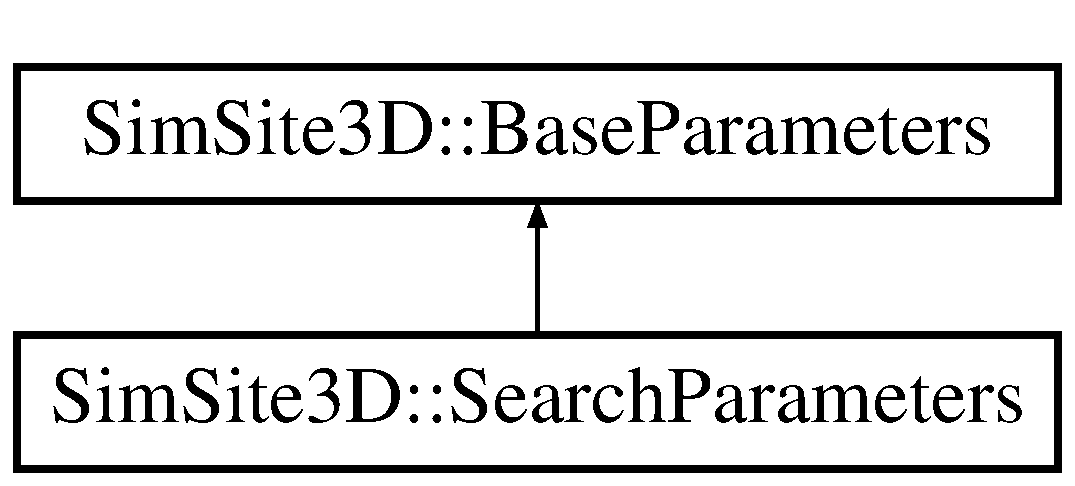
\includegraphics[height=2cm]{classSimSite3D_1_1SearchParameters}
\end{center}
\end{figure}
\subsection*{Public Types}
\begin{CompactItemize}
\item 
\textbf{PRINT\_\-VERSION} = 1\label{classSimSite3D_1_1SearchParameters_0278737369e96b0ca8d7685578a160d523d6d6cc3c507f57dbfb27c66de5af61}

\item 
\textbf{PRINT\_\-HELP}\label{classSimSite3D_1_1SearchParameters_0278737369e96b0ca8d7685578a160d5946fe3b6fb33a3f1a1f1bfcb799e7f57}

\item 
\textbf{DO\_\-NOT\_\-NORMALIZE}\label{classSimSite3D_1_1SearchParameters_0278737369e96b0ca8d7685578a160d56d064d2864a74b09ebb91ade006be98b}

\item 
\textbf{LIGAND\_\-RMSD}\label{classSimSite3D_1_1SearchParameters_0278737369e96b0ca8d7685578a160d539c302e55fa4a62c9fc42ddaf0aecf79}

\item 
\textbf{SITEMAP\_\-RMSD}\label{classSimSite3D_1_1SearchParameters_0278737369e96b0ca8d7685578a160d5be2fcd7debcbc43f9246f2e96a55b061}

\item 
\textbf{DO\_\-NOT\_\-WRITE\_\-LIGANDS}\label{classSimSite3D_1_1SearchParameters_0278737369e96b0ca8d7685578a160d5842ee3990d6101fe149155fb635857f8}

\item 
\textbf{SCORE\_\-ONLY}\label{classSimSite3D_1_1SearchParameters_0278737369e96b0ca8d7685578a160d56cca043172e95be1ac3a62aa07b3e929}

\item 
\textbf{DO\_\-NOT\_\-TIME\_\-PROCESS}\label{classSimSite3D_1_1SearchParameters_0278737369e96b0ca8d7685578a160d5df4956ce18d7222d72380e017a2f08a0}

\item 
\textbf{ALLOW\_\-HPHOB\_\-ONLY\_\-TRIANGLES}\label{classSimSite3D_1_1SearchParameters_0278737369e96b0ca8d7685578a160d5ff8d9bfbd20c4d153faebdc41c3a6850}

\item 
\textbf{ADD\_\-STRUCT\_\-ID\_\-FIELD}\label{classSimSite3D_1_1SearchParameters_0278737369e96b0ca8d7685578a160d57ed6e1e5168b8f6cc426662e6d3dcff8}

\item 
\textbf{DO\_\-PROT\_\-LIG\_\-SCORING}\label{classSimSite3D_1_1SearchParameters_0278737369e96b0ca8d7685578a160d58f07579b71a52c91abe56ecb74b4ff36}

\item 
\textbf{USE\_\-HBOND\_\-SURFACES\_\-MODEL}\label{classSimSite3D_1_1SearchParameters_0278737369e96b0ca8d7685578a160d5831a2cb95cee561617e96d228eafcedc}

\item 
\textbf{ALLOW\_\-SMALL\_\-SITEMAPS}\label{classSimSite3D_1_1SearchParameters_0278737369e96b0ca8d7685578a160d543f499df35fbe981319f676f9ed14378}

\item 
\textbf{OMIT\_\-SURFACES}\label{classSimSite3D_1_1SearchParameters_0278737369e96b0ca8d7685578a160d5e693337097e34cd00710717ddf730bf8}

\item 
\textbf{USE\_\-ONLY\_\-SURFACE\_\-TO\_\-RANK}\label{classSimSite3D_1_1SearchParameters_0278737369e96b0ca8d7685578a160d53000fed16c2b781a9796124b224878ee}

\item 
\textbf{NO\_\-FINE\_\-TUNING}\label{classSimSite3D_1_1SearchParameters_0278737369e96b0ca8d7685578a160d5411105460cac2fc65d5266f43736c78f}

\item 
\textbf{FINE\_\-TUNE\_\-TIER2\_\-ALIGNMENTS}\label{classSimSite3D_1_1SearchParameters_0278737369e96b0ca8d7685578a160d5ecbffd5cf9076e2f4f2d9c596905b669}

\item 
\textbf{FINE\_\-TUNE\_\-BEST\_\-TIER2\_\-ALIGNMENT}\label{classSimSite3D_1_1SearchParameters_0278737369e96b0ca8d7685578a160d504576ab0c5c8f5dbbba804c2c0274d2a}

\item 
\textbf{SAVE\_\-RIGID\_\-SCORES}\label{classSimSite3D_1_1SearchParameters_0278737369e96b0ca8d7685578a160d544f84bff804eec7f7c39354f9f8ae626}

\item 
\textbf{CHECK\_\-ALL\_\-TRIANGLES}\label{classSimSite3D_1_1SearchParameters_0278737369e96b0ca8d7685578a160d50f64c95335dd96cc5921f4fe06da140f}

\item 
\textbf{SCALE\_\-SF\_\-TERMS}\label{classSimSite3D_1_1SearchParameters_0278737369e96b0ca8d7685578a160d5760e17a2d0988a03d917adef472a93ed}

\item 
\textbf{IK\_\-SURFACES} = 1000\label{classSimSite3D_1_1SearchParameters_c267aed4ea246dc936ccd5b47b71712d64b3f0cd752f91d46f25e27e791c5bf6}

\item 
\textbf{IK\_\-HB\_\-CAPS}\label{classSimSite3D_1_1SearchParameters_c267aed4ea246dc936ccd5b47b71712d439d788290c8a2e8caad1e96753d001b}

\item 
\textbf{IK\_\-BOTH\_\-REPS}\label{classSimSite3D_1_1SearchParameters_c267aed4ea246dc936ccd5b47b71712d1aa6526aee8d82d030cda47ac9831efb}

\item 
enum \textbf{popt\_\-args\_\-t} \{ \par
\textbf{PRINT\_\-VERSION} =  1, 
\textbf{PRINT\_\-HELP}, 
\textbf{DO\_\-NOT\_\-NORMALIZE}, 
\textbf{LIGAND\_\-RMSD}, 
\par
\textbf{SITEMAP\_\-RMSD}, 
\textbf{DO\_\-NOT\_\-WRITE\_\-LIGANDS}, 
\textbf{SCORE\_\-ONLY}, 
\textbf{DO\_\-NOT\_\-TIME\_\-PROCESS}, 
\par
\textbf{ALLOW\_\-HPHOB\_\-ONLY\_\-TRIANGLES}, 
\textbf{ADD\_\-STRUCT\_\-ID\_\-FIELD}, 
\textbf{DO\_\-PROT\_\-LIG\_\-SCORING}, 
\textbf{USE\_\-HBOND\_\-SURFACES\_\-MODEL}, 
\par
\textbf{ALLOW\_\-SMALL\_\-SITEMAPS}, 
\textbf{OMIT\_\-SURFACES}, 
\textbf{USE\_\-ONLY\_\-SURFACE\_\-TO\_\-RANK}, 
\textbf{NO\_\-FINE\_\-TUNING}, 
\par
\textbf{FINE\_\-TUNE\_\-TIER2\_\-ALIGNMENTS}, 
\textbf{FINE\_\-TUNE\_\-BEST\_\-TIER2\_\-ALIGNMENT}, 
\textbf{SAVE\_\-RIGID\_\-SCORES}, 
\textbf{CHECK\_\-ALL\_\-TRIANGLES}, 
\par
\textbf{SCALE\_\-SF\_\-TERMS}
 \}
\item 
enum \textbf{IK\_\-type\_\-t} \{ \textbf{IK\_\-SURFACES} =  1000, 
\textbf{IK\_\-HB\_\-CAPS}, 
\textbf{IK\_\-BOTH\_\-REPS}
 \}
\end{CompactItemize}
\subsection*{Public Member Functions}
\begin{CompactItemize}
\item 
\bf{Search\-Parameters} ()\label{classSimSite3D_1_1SearchParameters_a08c1e2d66f1c849ba1fb003a6bc6b7f}

\begin{CompactList}\small\item\em To be used by the SimSite3D\-Py search.parameters module. \item\end{CompactList}\item 
\bf{Search\-Parameters} (const int argc, const char $\ast$$\ast$argv)\label{classSimSite3D_1_1SearchParameters_1acc5cc86e0834742971c7a66033c951}

\begin{CompactList}\small\item\em Set the search parameters using the values in argv. \item\end{CompactList}\item 
void \textbf{report\_\-parameters} (std::ostream \&out) const \label{classSimSite3D_1_1SearchParameters_c3a3ee055bce67d5d055a7a0a939c860}

\end{CompactItemize}
\subsection*{Public Attributes}
\begin{CompactItemize}
\item 
std::string \bf{ext\_\-score\_\-method}\label{classSimSite3D_1_1SearchParameters_31b913ee478296612756c9b25b34465d}

\begin{CompactList}\small\item\em Name of external scoring method to use. \item\end{CompactList}\item 
std::string \bf{model\_\-file\_\-name}\label{classSimSite3D_1_1SearchParameters_cdcb30f0c043a4137ed8c790502ada62}

\begin{CompactList}\small\item\em Name of the model points file. \item\end{CompactList}\item 
std::string \bf{dbase\_\-file\_\-name}\label{classSimSite3D_1_1SearchParameters_c70448bc467a512efafbf3b952770550}

\begin{CompactList}\small\item\em Name of the current dbase points file. \item\end{CompactList}\item 
std::string \bf{ofname}\label{classSimSite3D_1_1SearchParameters_51c7063e6085b9aa32527a64206ecfdc}

\begin{CompactList}\small\item\em Name of the output file. \item\end{CompactList}\item 
std::string \bf{score\_\-str}\label{classSimSite3D_1_1SearchParameters_770e3c6ff6ae15a21330d15dcfe3d4d5}

\begin{CompactList}\small\item\em Scoring method. \item\end{CompactList}\item 
std::string \bf{db\_\-index\_\-fname}\label{classSimSite3D_1_1SearchParameters_48d9df89d360efd9b57b8917aae33712}

\begin{CompactList}\small\item\em Name of database index file. \item\end{CompactList}\item 
int \bf{db\_\-start}\label{classSimSite3D_1_1SearchParameters_2cd53037b00008f5039381a00085f93d}

\begin{CompactList}\small\item\em Line number of initial db site. \item\end{CompactList}\item 
int \bf{db\_\-stop}\label{classSimSite3D_1_1SearchParameters_b12f931a64c6d18141bb94cb283c1543}

\begin{CompactList}\small\item\em Line number of final db site. \item\end{CompactList}\item 
bool \bf{normalize}\label{classSimSite3D_1_1SearchParameters_4265eb5c3b8cd524159bcefd855458fa}

\begin{CompactList}\small\item\em false implies no normalization \item\end{CompactList}\item 
int \bf{num\_\-scores\_\-to\_\-keep}\label{classSimSite3D_1_1SearchParameters_275f0141e87e686c4c8ee55d9062ae81}

\begin{CompactList}\small\item\em max \# of final alignments to keep for each search sitemap \item\end{CompactList}\item 
int \bf{max\_\-tier1\_\-aligns}\label{classSimSite3D_1_1SearchParameters_d8fa144982e1f3a459b6797170fec1e9}

\begin{CompactList}\small\item\em max \# of tier1 alignments to pass to tier2 scoring \item\end{CompactList}\item 
my\_\-float\_\-t \bf{score\_\-cutoff}\label{classSimSite3D_1_1SearchParameters_2ee1752f506f23f99dc8639465c83015}

\begin{CompactList}\small\item\em Keep alignments with score better than cutoff. \item\end{CompactList}\item 
int \bf{min\_\-num\_\-atoms}\label{classSimSite3D_1_1SearchParameters_b82481de1a76a7e1ef2701225f4e8e2b}

\begin{CompactList}\small\item\em Number of ligand atoms required in query pocket. \item\end{CompactList}\item 
my\_\-float\_\-t \bf{dmetol}\label{classSimSite3D_1_1SearchParameters_9afa8f1e64a425ad8e45aaf7402029c7}

\begin{CompactList}\small\item\em Tolerance for the average dist. metric error. \item\end{CompactList}\item 
my\_\-float\_\-t \bf{lsetol}\label{classSimSite3D_1_1SearchParameters_fd82cd2d31ed05774d10ab78235133f6}

\begin{CompactList}\small\item\em Tolerance for the average least squares error. \item\end{CompactList}\item 
bool \textbf{ligand\_\-rmsd}\label{classSimSite3D_1_1SearchParameters_922b10578a528a00d7b98686005636fe}

\item 
bool \textbf{sitemap\_\-rmsd}\label{classSimSite3D_1_1SearchParameters_bfcbc6418735f08eb7d0f7bd11d12a62}

\item 
bool \bf{write\_\-ligands}\label{classSimSite3D_1_1SearchParameters_8f581cefd00526d81c5db9e7f2e53dd7}

\begin{CompactList}\small\item\em True implies write ligands, else do not write. \item\end{CompactList}\item 
bool \bf{align\_\-to\_\-query}\label{classSimSite3D_1_1SearchParameters_1cb575b033f4db440a377d4ea8332929}

\begin{CompactList}\small\item\em True implies align dbase site to query, else score as given. \item\end{CompactList}\item 
size\_\-t \bf{num\_\-rand\_\-aligns}\label{classSimSite3D_1_1SearchParameters_019cff6f0e6b9d6028f7e9fab62e62b6}

\begin{CompactList}\small\item\em If not align\_\-to\_\-query, use this many random alignments. \item\end{CompactList}\item 
bool \bf{time\_\-process}\label{classSimSite3D_1_1SearchParameters_7ed54b1f8513ddd3e56686c36fb0f89d}

\begin{CompactList}\small\item\em If true, use itimers to time program. \item\end{CompactList}\item 
bool \bf{allow\_\-hphob\_\-triangles}\label{classSimSite3D_1_1SearchParameters_a9d1bb630cda4fe759f4299354cef05f}

\begin{CompactList}\small\item\em If false, triangle need at least 1 hbond. \item\end{CompactList}\item 
bool \bf{add\_\-struct\_\-id\_\-field}\label{classSimSite3D_1_1SearchParameters_6dbd7bf284c1dbfd2c2af2becf89a078}

\begin{CompactList}\small\item\em If false \& empty pockets searches, write struct id into ligand field for empty pocket hits. \item\end{CompactList}\item 
bool \bf{do\_\-internal\_\-prot\_\-lig\_\-score}\label{classSimSite3D_1_1SearchParameters_96a5af359501d56a5670d49c32467994}

\begin{CompactList}\small\item\em If true compute affi and orient score for query prot and db lig interactions. \item\end{CompactList}\item 
bool \bf{use\_\-hbond\_\-surfaces}\label{classSimSite3D_1_1SearchParameters_1c517ad691e1606cce4cdfac986067b0}

\begin{CompactList}\small\item\em If true, use the hbond surfaces modeling of hydrogen bonding regions (volumes). \item\end{CompactList}\item 
bool \bf{fine\_\-tune\_\-tier2\_\-alignments}\label{classSimSite3D_1_1SearchParameters_7e249d3358f464048cca7f574052e844}

\begin{CompactList}\small\item\em If true, use an ICP like method to fine tune all tier2 alignments. \item\end{CompactList}\item 
bool \bf{fine\_\-tune\_\-best\_\-tier2\_\-alignment}\label{classSimSite3D_1_1SearchParameters_6c449d3293b369f0c71e875e14d2039a}

\begin{CompactList}\small\item\em If true, use an ICP-like method to fine tune the best scoring tier2 alignment. \item\end{CompactList}\item 
bool \bf{check\_\-all\_\-triangles}\label{classSimSite3D_1_1SearchParameters_44592b748c47ab06a54c680635dc0795}

\begin{CompactList}\small\item\em If true, check all triangles in dbase mesh for closest point to each query vertex -- useful for testing. \item\end{CompactList}\item 
std::string \bf{query\_\-prot}\label{classSimSite3D_1_1SearchParameters_600f1a2e9136a1c54dc751c3bc6f3665}

\begin{CompactList}\small\item\em Currently required for hbond\_\-surfaces. \item\end{CompactList}\item 
bool \bf{save\_\-rigid\_\-scores}\label{classSimSite3D_1_1SearchParameters_bc80a6f5d0264c5f4b5ca582c1183a14}

\begin{CompactList}\small\item\em When using ICP, save the rigid scores to another output file. \item\end{CompactList}\item 
bool \bf{scale\_\-terms}\label{classSimSite3D_1_1SearchParameters_dcb623f26a6aabaf855021f954cee078}

\begin{CompactList}\small\item\em If true, scale each term of the scoring function(s) linearly from [0.0, max] to [0.0, 1.0] where max is the max value the query site can have for that term. \item\end{CompactList}\item 
bool \textbf{do\_\-IK}\label{classSimSite3D_1_1SearchParameters_ae98a5075be2f4c92734f47223076e6c}

\item 
my\_\-float\_\-t \bf{max\_\-corr\_\-surf\_\-pt\_\-dist}\label{classSimSite3D_1_1SearchParameters_ac2413e22df6100db6b73f5920cc9ddd}

\begin{CompactList}\small\item\em Maximum distance to consider corresponding surface points. \item\end{CompactList}\item 
my\_\-float\_\-t \bf{fine\_\-tune\_\-ratio}\label{classSimSite3D_1_1SearchParameters_62849cae5f51eb12263a341056af66c5}

\begin{CompactList}\small\item\em Ratio of shape point weight (msms surf) to hbond cap point weight (1.0 imples equal, 2.0 implies surface points get weighted twice that of hbond caps, etc.) Default is Zero, which implies use only the MSMS surface for ICP. \item\end{CompactList}\item 
std::string \bf{alignments\_\-fname}\label{classSimSite3D_1_1SearchParameters_5a36fe41006109a902194d9e2cf39e1a}

\begin{CompactList}\small\item\em Path to alignments file (in Sim\-Site3D results file format with at least 4 fields per line -- struct\_\-id, score, R, T; and in that order and pipe delimited fields with numbers single space delimited). \item\end{CompactList}\item 
IK\_\-type\_\-t \bf{IK\_\-type}\label{classSimSite3D_1_1SearchParameters_84a374fa89c1f6d5868a830091d2178c}

\begin{CompactList}\small\item\em Type of IK method to use. \item\end{CompactList}\end{CompactItemize}
\subsection*{Private Member Functions}
\begin{CompactItemize}
\item 
void \textbf{init\_\-vars} ()\label{classSimSite3D_1_1SearchParameters_0b3092dc843090100b6d8707f438ff82}

\item 
void \textbf{free\_\-cstrings} ()\label{classSimSite3D_1_1SearchParameters_c5be044fd7c950fbf1b3472d01e9c0f5}

\item 
status\_\-t \textbf{get\_\-opts} (const int argc, const char $\ast$$\ast$argv)\label{classSimSite3D_1_1SearchParameters_e7af633b8fc93087ddf5067551929741}

\item 
status\_\-t \textbf{verify\_\-parameters} ()\label{classSimSite3D_1_1SearchParameters_cc0d8f138dd11fa98a0fa52c59f1a9b2}

\end{CompactItemize}
\subsection*{Private Attributes}
\begin{CompactItemize}
\item 
char $\ast$ \bf{A\_\-conf\_\-fname}\label{classSimSite3D_1_1SearchParameters_3cb03731b1e4917864cade8bb39d7f95}

\begin{CompactList}\small\item\em Location of environment configure file. \item\end{CompactList}\item 
char $\ast$ \bf{A\_\-proj\_\-output}\label{classSimSite3D_1_1SearchParameters_b89a1895609e2d782727d5b81e70fff4}

\begin{CompactList}\small\item\em Directory to store results. \item\end{CompactList}\item 
char $\ast$ \bf{A\_\-scratch\_\-dir}\label{classSimSite3D_1_1SearchParameters_27e0256e5782174a8a5da589e84ef6da}

\begin{CompactList}\small\item\em Directory to use as a scratch space. \item\end{CompactList}\item 
char $\ast$ \bf{A\_\-dbase\_\-dir}\label{classSimSite3D_1_1SearchParameters_2cbe4df7b590f7cb0fff7584fcecf59b}

\begin{CompactList}\small\item\em Location of the database to query. \item\end{CompactList}\item 
char $\ast$ \bf{A\_\-ligs\_\-dir}\label{classSimSite3D_1_1SearchParameters_3dc1434fb48a7773cbe4fd247a87de77}

\begin{CompactList}\small\item\em Location of ligands associated with dbase\_\-dir. \item\end{CompactList}\end{CompactItemize}
\subsection*{Static Private Attributes}
\begin{CompactItemize}
\item 
static const std::string \bf{A\_\-fname} = \char`\"{}Search\-Parameters.C\char`\"{}\label{classSimSite3D_1_1SearchParameters_865031ac44a12f4833a96bf17e718b2c}

\begin{CompactList}\small\item\em Name of the source file. \item\end{CompactList}\end{CompactItemize}


\subsection{Detailed Description}
Use popt to parse a search's commandline parameters. 



The documentation for this class was generated from the following files:\begin{CompactItemize}
\item 
Search\-Parameters.H\item 
Search\-Parameters.C\end{CompactItemize}
